%%% packages %%%
%%%%%%%%%%%%%%%%%%%%%%%%%%%%%%%%%%%%%%%%%%%%%%%%%%%%%%%%%%%%%%%%%%%%%%%%%%%%%%%  
\documentclass[frenchb]{report}
%\usepackage{natbib}
\usepackage{hyperref}
\usepackage[toc,page]{appendix}
\usepackage[dvipsnames]{xcolor}
\usepackage[french]{babel}
\usepackage{url}
\usepackage[utf8x]{inputenc}
\usepackage{graphicx}
\graphicspath{{images/}}
\usepackage{parskip}
\usepackage{fancyhdr}
\usepackage{fancyvrb}
\usepackage{vmargin}
\usepackage{xcolor}
\usepackage{bbm}
\usepackage{amsmath,amssymb}
\usepackage{amsthm}
\usepackage{dsfont}
\usepackage{stmaryrd}
\usepackage{systeme}
\usepackage{enumitem}
\usepackage{xcolor}
\usepackage{pifont}
\usepackage{textcomp}
\usepackage{calrsfs}
\usepackage[T1]{fontenc}
\usepackage[toc,page]{appendix}
\usepackage{lipsum}
\usepackage{verbatim}
\usepackage{listings}
\usepackage{adforn}
\usepackage{float}
\usepackage{subfig}
\RequirePackage{listings}% Pour incorporer du code dans un langage de programmation

%%%  MARGE   %%%%%%%%%%%%%%%%%%%%%%%%%%%%%%%%%%%%%%%%%%%%%%%%%%%%%%%%%%%%

\setlength{\hoffset}{-18pt}        
\setlength{\oddsidemargin}{0pt} % Marge gauche sur pages impaires
\setlength{\evensidemargin}{9pt} % Marge gauche sur pages paires
\setlength{\marginparwidth}{54pt} % Largeur de note dans la marge
\setlength{\textwidth}{481pt} % Largeur de la zone de texte (17cm)
\setlength{\voffset}{-18pt} % Bon pour DOS
\setlength{\marginparsep}{7pt} % Séparation de la marge
\setlength{\topmargin}{-25pt} % Pas de marge en haut
\setlength{\headheight}{0pt} % Haut de page
\setlength{\headsep}{10pt} % Entre le haut de page et le texte
\setlength{\footskip}{27pt} % Bas de page + séparation
\setlength{\textheight}{720pt} % Hauteur de la zone de texte (25cm)

%%%%%%%%%%%%%%%%%%%%%%%%%%%%%%%%%%%%%%%%%%%%%%%%%%%%%%%%%%%%

\makeatletter
\let\thetitle\@title
\let\theauthor\@author
\let\thedate\@date
\makeatother

%%% commandes mise en page %%%
%%%%%%%%%%%%%%%%%%%%%%%%%%%%%%%%%%%%%%%%%%%%%%%%%%%%%%%%%%%%%%%%%%%%%%%%%%%%%%%        
\newcommand{\ld}{\log_{2}}
\newcommand{\R}{\mathbbm{R}}
\newcommand{\N}{\mathbbm{N}}
\newcommand{\1}{\mathbbm{1}}
\newcommand{\E}{\mathbbm{E}}
\newcommand{\V}{\mathbbm{V}}
\newcommand{\prob}{\mathbbm{P}}
\newcommand{\Nc}{\mathcal{N}}
\newcommand{\Cc}{\mathcal{C}}
\newcommand{\K}{\mathcal{K}}
\newcommand{\Xti}{\widetilde{X_i}}
\newcommand{\Xtj}{\widetilde{X_j}}
\newcommand{\Xn}{\overline{X_n}}
\newcommand{\gn}{\hat{g_n}}
\newcommand{\n}{\mathcal{N}}
\newcommand{\lv}{\mathcal{L}}
\newcommand{\thetat}{\tilde{\theta}}

\newcommand{\console}[1]{\colorbox{black}{\begin{minipage}[c]{1\linewidth}\textcolor{white}{\texttt{#1}}\end{minipage}}}

\newtheorem{prop}{Proposition}
\newtheorem{thm}{Théorème}
\newtheorem{cor}{Corollaire}
\newtheorem{lem}{Lemme}
\newtheorem{hyp}{Hypothèse}
\theoremstyle{definition}\newtheorem{defn}{Définition}
\theoremstyle{definition}\newtheorem{exm}{Exemple}
\theoremstyle{definition}\newtheorem{nota}{Notation}
\theoremstyle{definition}\newtheorem{rem}{Remarque}

\renewcommand{\qedsymbol}{\adfhangingflatleafright}

% pour incorporer le code dans le rapport
\lstdefinelanguage{Python}%
{morekeywords={import,function,for,in,if,elseif,else,true,false,end,%
		return,while,as,len,enumerate,print,range,%
		edges,src,dst,has_edge,isempty,size,zeros,minimum,},%
	sensitive=true,%
	morecomment=[n]{\#},%
	morestring=[s]{"}{"},%
	morestring=[m]{'}{'},%
}[keywords,comments,strings]%

\lstset{%
	language         = Python,
	basicstyle       = \ttfamily,
	keywordstyle     = \bfseries\color{blue},
	stringstyle      = \color{magenta},
	commentstyle     = \color{green},
	showstringspaces = false,
}

\begin{document}
%%% Pour l'annexe
\def\appendixpage{\vspace*{8cm}
\begin{center}
\Huge\textbf{Annexes}
\end{center}
}
\def\appendixname{Annexe}%

\begin{titlepage}
\begin{center}

\includegraphics[scale=0.6]{images/logo.png}
\hfill

\includegraphics[scale=0.35]{images/fds_logo.png}
\hfill

\includegraphics[scale=0.30]{images/ssd.png}\\[3cm]
\linespread{1.2}\huge {\bfseries Apprentissage Statistique }\\[0.5cm]
\linespread{1.2}\LARGE {\bfseries TP n°5 : Perceptron multicouche}\\[1.5cm]
\linespread{1}

{\large Rédigé par\\}
{\Large \textsc{CÔME Olivier} }\\
{\Large \textsc{PRALON} Nicolas}\\
{\Large \textsc{SENE} Assane}\\[1cm]


\includegraphics[scale=0.7]{images/imag_logo.png}

\end{center}
\end{titlepage}
%%%%%%%%%%%%%%%%%%%%%%%%%%%%%%%%%%%%%%%%%%%%%%%%%%%%%%%%%%%%%%%%%%%%%%%%%%%%%%%%%%%%%%%%%
\tableofcontents
\newpage
%%%%%%%%%%%%%%%%%%%%%%%%%%%%%%%%%%%%%%%%%%%%%%%%%%%%%%%%%%%%%%%%%%%%%%%%%%%%%%%%%%%%%%%%%

\chapter*{Introduction}
\addcontentsline{toc}{part}{Introduction}

\section*{Question 1}

\addcontentsline{toc}{part}{Question 1}

\underline{Présentons très synthétiquement le jeu de données pour le \textit{AND}, \textit{XOR} et \textit{OR}:}

\begin{figure}[htp] 
	\centering
	\subfloat[Graphique du jeu de données \textit{AND}]{%
		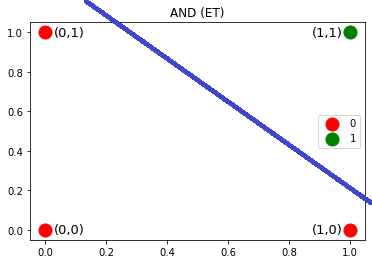
\includegraphics[scale=1.1]{images/AND.png}%
	}%
	\hfill%
	\subfloat[Graphique du jeu de données \textit{XOR}]{%
		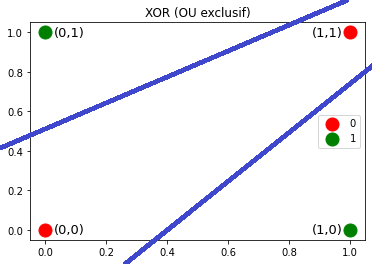
\includegraphics[scale=1.1]{images/XOR.png}%
	}%
	\hfill%
	\subfloat[Graphique du jeu de données \textit{OR}]{%
		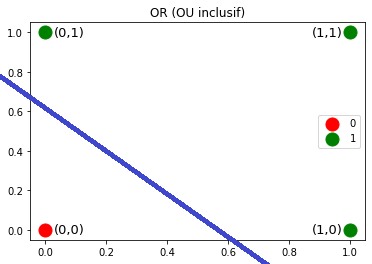
\includegraphics[scale=1.1]{images/OR.png}%
	}%
\end{figure}
Les difficultés de classification résident dans le fait que les données du \textit{XOR} ne sont pas linéairement séparables. Sur le graphique (b) on voit qu'il y a deux droites de séparation et non une seule. De ce fait, un seul neurone ne peut réussir à classifier les données.

\section*{Question 2}

\addcontentsline{toc}{part}{Question 2}

\underline{Définissons un classifieur \textit{MLP} pour apprendre l’opérateur \textit{AND}:}

\begin{figure}[H]
	\centering
	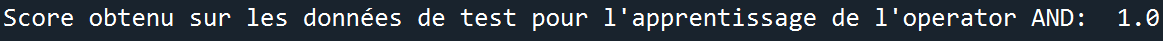
\includegraphics[scale=0.7]{images/Q2.png}
	\caption{Score obtenu par le classifieur $MLP$ sur les données de test de l'opérateur $AND$}
\end{figure}
Dans le cas où l'on souhaite apprendre l'opérateur $AND$, le classifieur $MLP$ ne comprenant aucune couche cachée fournit de très bons résultats en terme de prédiction. Comme on peut le voir sur la figure 1, le classifieur ne fait aucune erreur de prédiction (le score vaut $1$). Pour calculer ce score nous avons utiliser la fonction $score(x\_test, y\_test)$ de $sklearn$.
\section*{Question 3}

\addcontentsline{toc}{part}{Question 3}

\underline{Définissons un classifieur \textit{MLP} pour apprendre l’opérateur \textit{OR}:}

\begin{figure}[H]
	\centering
	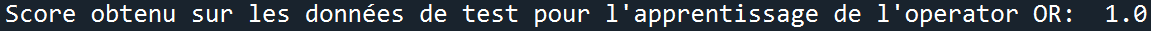
\includegraphics[scale=0.7]{images/Q3.png}
	\caption{Score obtenu par le classifieur $MLP$ sur les données de test de l'opérateur $OR$}
\end{figure}
Dans le cas où l'on souhaite apprendre l'opérateur $OR$, le classifieur $MLP$ ne comprenant aucune couche cachée fournit de très bons résultats en terme de prédiction. Comme on peut le voir sur la figure 2, le classifieur ne fait aucune erreur de prédiction (le score vaut $1$). Pour calculer ce score nous avons utiliser la fonction $score(x\_test, y\_test)$ de $sklearn$.

\section*{Question 4}
\addcontentsline{toc}{part}{Question 3}
\subsection{a)}

\underline{Définissons un classifieur \textit{MLP} sans couche cachée pour apprendre l’opérateur \textit{XOR}:}

\begin{figure}[H]
	\centering
	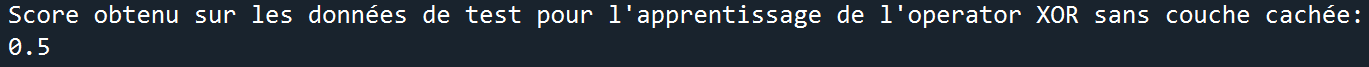
\includegraphics[scale=0.7]{images/Q4a.png}
	\caption{Score obtenu par le classifieur $MLP$ sur les données de test de l'opérateur $XOR$ sans utiliser de couches cachées}
\end{figure}
Dans le cas où l'on souhaite apprendre l'opérateur $XOR$, le classifieur $MLP$ ne comprenant aucune couche cachée fournit de mauvais résultats en terme de prédiction. Comme on peut le voir sur la figure 3, la précision de prédiction du classifieur est de $50\%$ (le score vaut $0.5$), ce qui est assez bas.\\
Cela s'explique par le fait qu'un perceptron ne peut apprendre que sur des données linéairement séparables or ce n'est ici pas le cas.
\addcontentsline{toc}{part}{Question 4}

\subsection{b)}

\underline{Définissons un classifieur \textit{MLP} avec deux couches cachées pour apprendre l’opérateur \textit{XOR}:}


\begin{figure}[H]
	\centering
	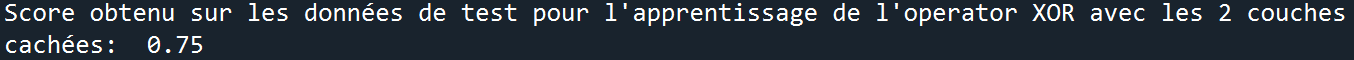
\includegraphics[scale=0.7]{images/Q4b.png}
	\caption{Score obtenu par le classifieur $MLP$ sur les données de test de l'opérateur $XOR$ en utilisant $2$ couches cachées}
\end{figure}
Le classifieur $MLP$ comprenant deux couches cachées ($4$ neurones sur la première couche et $2$ neurones sur la deuxième) fournit de meilleurs résultats (en terme de prédiction) que le classifieur ne comprenant aucune couche cachée. En effet, comme on peut le voir sur la figure 4, la précision de prédiction de ce nouveau classifieur est de $75\%$ contre $50\%$ pour le précédent.\\
Cela s'explique par le fait que l'ajout de couches cachées dans un perceptron permet de transformer un problème non linéairement séparable en un problème linéairement séparable. Ce nouveau classifieur (perceptron multi-couche) sera donc en mesure d'apprendre l'opérateur XOR contrairement au précèdent.

\subsection{c)}

\underline{Classifieur \textit{MLP} avec deux couches cachées et des fonctions d'activation hyperbolique pour apprendre l’opérateur \textit{XOR}:}

\begin{figure}[H]
	\centering
	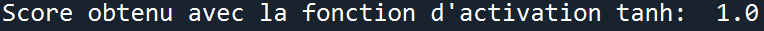
\includegraphics[scale=0.7]{images/Q4c.png}
	\caption{Score obtenu par le classifieur $MLP$ sur les données de test de l'opérateur $XOR$ en utilisant $2$ couches cachées et des fonctions d'activation $tanh$}
\end{figure}
Les résultats obtenus ici sont encore mieux que ceux obtenus dans les deux cas précédents. En effet, comme on peut le voir sur la figure 5, la précision de prédiction de ce nouveau classifieur est de $100\%$ contre $75\%$ et $50\%$ pour les deux précédents.
Les fonctions d'activation hyperbolique ($tanh$) cherchent des séparateurs non linéaires or nos données sont ici non linéairement séparables. Par conséquent, ces fonctions d'activation seront bien adaptées à notre situation. Cela explique pourquoi les résultats obtenus ici sont mieux que ceux obtenus précédemment.

\section*{Question 5}

\addcontentsline{toc}{part}{Question 5}

Notre jeu de donnée est composé d'images (de taille 8$\times$8 c'est à dire $64$ pixels) de chiffre manuscrit. On veut identifier le chiffre contenu dans une image. On cherche donc ici à mettre en place un réseau de neurones qui sera capable de classifier ces images. Étant donné qu'il y a $10$ chiffres allant de $0$ à $9$, nous aurons ici un nombre total de $10$ classes.\\\\

Nous allons comparer les performances de plusieurs classifieur que nous aurons crée en jouant sur différents paramètres de $MLPclassifieur$. Nous regrouperons ces performances dans un tableau puis nous regarderons quel classifieur fournit les meilleurs performances.

\begin{figure}[htp] 
	\centering
	\subfloat[Dataframe des scores des différents classifieurs utilisés]{%
		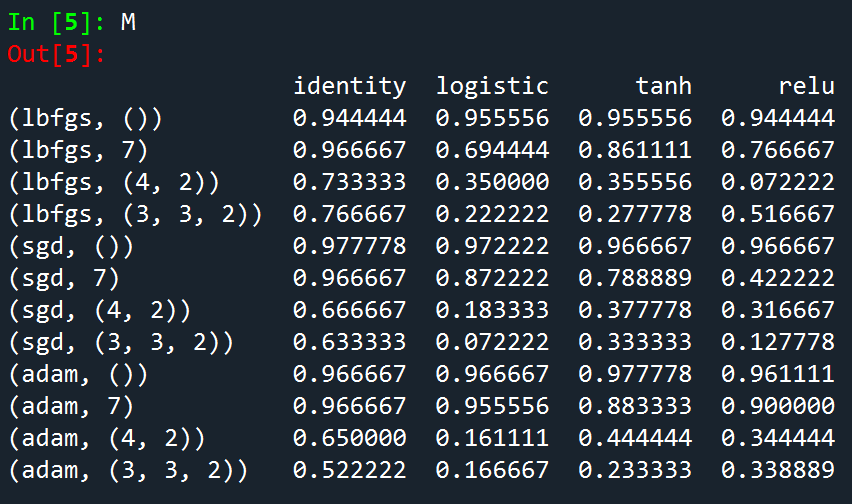
\includegraphics[scale=0.65]{images/df_MLP.png}%
	}%
	\hfill%
	\subfloat[Meilleurs $MLP$ en fonctions des différentes fonctions d'activations]{%
		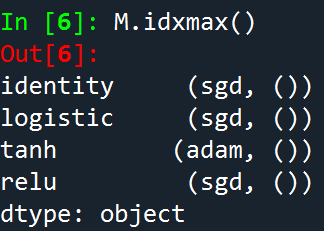
\includegraphics[scale=1.4]{images/best_MLP.png}%
	}%
	\caption{}
\end{figure}

D'après la figure $6$, on constate que les classifieurs sans couches cachées sont les plus performant. Ce résultat est étonnant puisqu'ici, les données sont linéairement non séparables. Les classifieurs $MLP$ ayant les meilleurs performances sont ceux ayant pour fonctions d'activation la fonction tangente hyperbolique ($tanh$) et la fonction linéaire ($identity$). Étant donné que les données sont linéairement non séparables, on se serait plutôt attendu à avoir de meilleurs résultats avec la fonction d'activation $tanh$ et l'optimiseur $adam$.

\section*{Question 6}

\addcontentsline{toc}{part}{Question 6}

\begin{figure}[H]
	\centering
	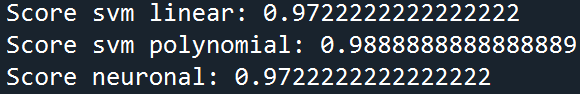
\includegraphics[scale=0.7]{images/SVM_vs_MLP.png}
	\caption{Comparaison entre le classifieur $SVM$ et $MLP$}
\end{figure}

Dans cette dernière question nous comparons le classifieur $MLP$ obtenu dans la question précédente avec deux classifieurs $SVM$. Afin de déterminer le meilleur de ces trois classifieur, nous évaluons les performances des deux classifieur $SVM$ en validation croisé avec un k-fold (k = 5).\\
D'après la figure $7$, on constate que le classifieur $SVM$ avec le noyau polynomial est le meilleur car c'est celui ayant le score le plus élevé.


\end{document}